\begin{center}
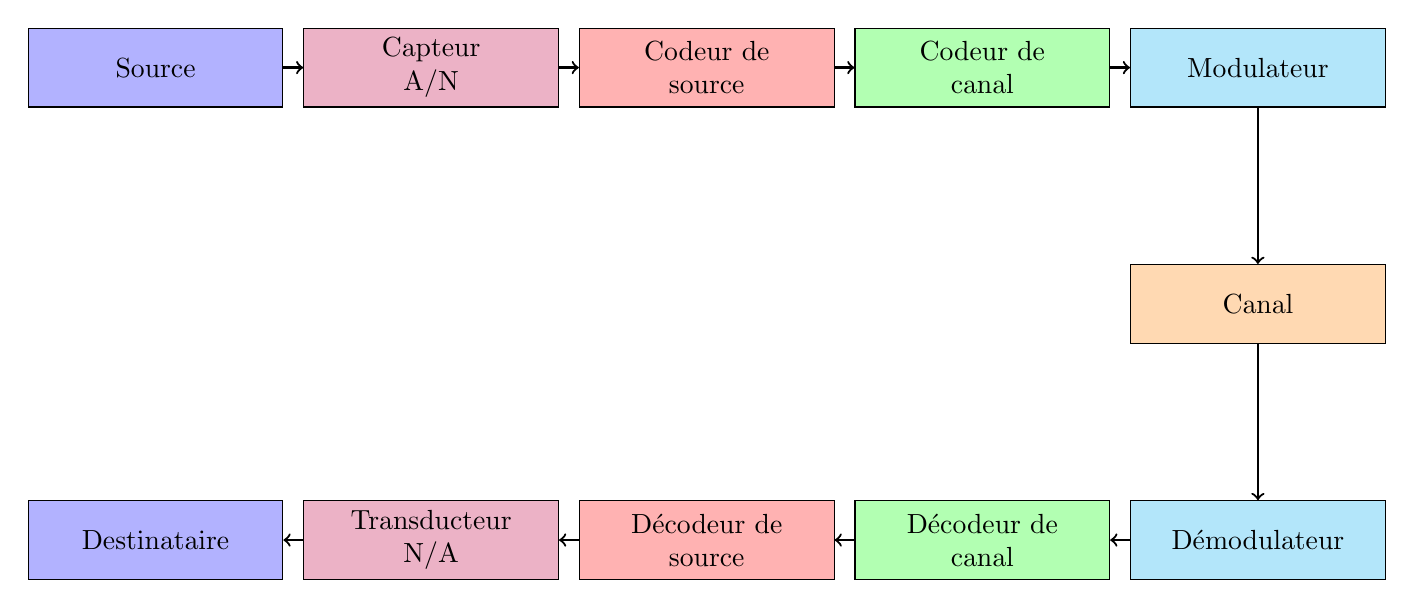
\begin{tikzpicture}[node distance=3cm, auto]

% Define styles
\tikzstyle{block} = [draw, rectangle, minimum width=3cm, minimum height=1cm, text centered, text width=3cm]
\tikzstyle{line} = [->, thick]

% First row
\node[block, fill=blue!30] (source) {Source};
\node[block, fill=purple!30, right of=source, xshift=0.5cm] (adc) {Capteur\\A/N};
\node[block, fill=red!30, right of=adc, xshift=0.5cm] (encoder) {Codeur de\\source};
\node[block, fill=green!30, right of=encoder, xshift=0.5cm] (channelencoder) {Codeur de\\canal};
\node[block, fill=cyan!30, right of=channelencoder, xshift=0.5cm] (modulator) {Modulateur};

% Second row
\node[block, fill=orange!30, below of=modulator, node distance=3cm] (channel) {Canal};

% Third row
\node[block, fill=cyan!30, below of=channel, node distance=3cm] (demodulator) {Démodulateur};
\node[block, fill=green!30, left of=demodulator, xshift=-0.5cm] (channeldecoder) {Décodeur de\\canal};
\node[block, fill=red!30, left of=channeldecoder, xshift=-0.5cm] (decoder) {Décodeur de\\source};
\node[block, fill=purple!30, left of=decoder, xshift=-0.5cm] (dac) {Transducteur\\N/A};
\node[block, fill=blue!30, left of=dac, xshift=-0.5cm] (destination) {Destinataire};

% Arrows
\draw[line] (source) -- (adc);
\draw[line] (adc) -- (encoder);
\draw[line] (encoder) -- (channelencoder);
\draw[line] (channelencoder) -- (modulator);
\draw[line] (modulator) -- (channel);
\draw[line] (channel) -- (demodulator);
\draw[line] (demodulator) -- (channeldecoder);
\draw[line] (channeldecoder) -- (decoder);
\draw[line] (decoder) -- (dac);
\draw[line] (dac) -- (destination);

\end{tikzpicture}
\end{center}



\begin{center}
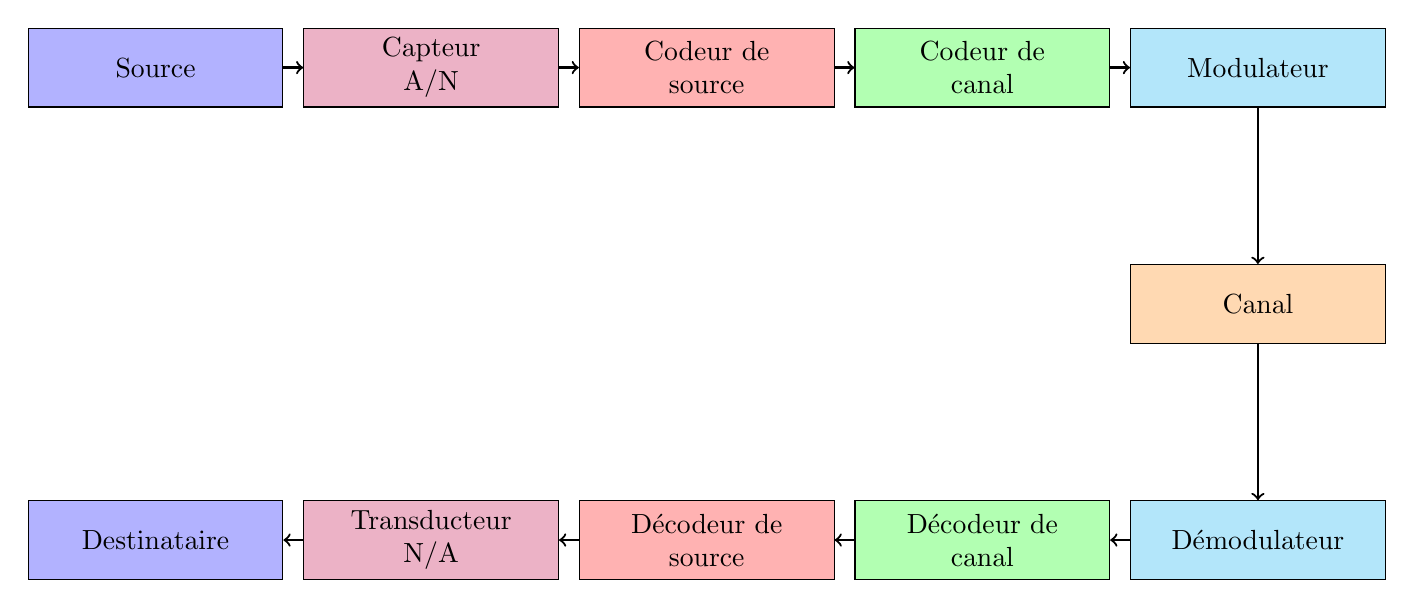
\begin{tikzpicture}[node distance=3cm, auto]

% Define styles
\tikzstyle{block} = [draw, rectangle, minimum width=3cm, minimum height=1cm, text centered, text width=3cm]
\tikzstyle{line} = [->, thick]

% First row
\node[block, fill=blue!30] (source) {Source};
\node[block, fill=purple!30, right of=source, xshift=0.5cm] (adc) {Capteur\\A/N};
\node[block, fill=red!30, right of=adc, xshift=0.5cm] (encoder) {Codeur de\\source};
\node[block, fill=green!30, right of=encoder, xshift=0.5cm] (channelencoder) {Codeur de\\canal};
\node[block, fill=cyan!30, right of=channelencoder, xshift=0.5cm] (modulator) {Modulateur};

% Second row
\node[block, fill=orange!30, below of=modulator, node distance=3cm] (channel) {Canal};

% Third row
\node[block, fill=cyan!30, below of=channel, node distance=3cm] (demodulator) {Démodulateur};
\node[block, fill=green!30, left of=demodulator, xshift=-0.5cm] (channeldecoder) {Décodeur de\\canal};
\node[block, fill=red!30, left of=channeldecoder, xshift=-0.5cm] (decoder) {Décodeur de\\source};
\node[block, fill=purple!30, left of=decoder, xshift=-0.5cm] (dac) {Transducteur\\N/A};
\node[block, fill=blue!30, left of=dac, xshift=-0.5cm] (destination) {Destinataire};

% Arrows
\draw[line] (source) -- (adc);
\draw[line] (adc) -- (encoder);
\draw[line] (encoder) -- (channelencoder);
\draw[line] (channelencoder) -- (modulator);
\draw[line] (modulator) -- (channel);
\draw[line] (channel) -- (demodulator);
\draw[line] (demodulator) -- (channeldecoder);
\draw[line] (channeldecoder) -- (decoder);
\draw[line] (decoder) -- (dac);
\draw[line] (dac) -- (destination);

\end{tikzpicture}
\caption{Overleaf logo}
\end{center}

